\documentclass[aspectratio=169,11pt]{beamer}

% ---------- theme ----------
\usetheme{Madrid}
\usecolortheme{whale}
\useinnertheme{circles}
\setbeamertemplate{navigation symbols}{}
\setbeamertemplate{caption}[numbered]
\usepackage{lmodern}
\usepackage[T1]{fontenc}
\usepackage{booktabs}
\usepackage{colortbl}   % for \rowcolor in tables
\usepackage{tikz}
\usetikzlibrary{arrows.meta,positioning,shapes.geometric,fit,backgrounds}
\usepackage{xcolor}

\definecolor{rbblue}{RGB}{18,72,120}
\definecolor{rbaccent}{RGB}{200,60,55}
\definecolor{rbgreen}{RGB}{28,120,80}
\definecolor{rbgray}{RGB}{90,90,90}
\setbeamercolor{structure}{fg=rbblue}
\setbeamercolor{block title}{bg=rbblue,fg=white}
\setbeamercolor{block title alerted}{bg=rbaccent,fg=white}
\setbeamercolor{block title example}{bg=rbgreen,fg=white}

\newcommand{\rsr}{\mbox{RSR@5}}
\newcommand{\good}[1]{\textcolor{rbgreen}{\textbf{#1}}}
\newcommand{\bad}[1]{\textcolor{rbaccent}{\textbf{#1}}}

% ---------- title ----------
\title[Retrieval-Barrier IPI: Attack \& Defense]{Overcoming the Retrieval Barrier}
\subtitle{Reproducing Retrieval-Stage Indirect Prompt Injection\\and Building a Provenance-Aware Defense}
\author[Tareq \& Shafee]{Sadman Bin Tareq (2105040) \and Rageeb Hasan Shafee (2105175)}
\institute[]{Project progress report\\\footnotesize Based on Chang, Bao, Luo, Yu --- \emph{Overcoming the Retrieval Barrier: IPI in the Wild for LLM Systems}, USENIX Security 2026 (arXiv:2601.07072)}
\date{\today}

\begin{document}

\begin{frame}[plain]
  \titlepage
\end{frame}

\begin{frame}{Outline}
  \tableofcontents
\end{frame}

% ===================================================================
\section{Background and Threat Model}

\begin{frame}{The retrieval barrier in one picture}
  \small
  Modern LLM assistants are \textbf{retrieval-augmented (RAG)}: they fetch the top-$k$ most relevant documents and read them before answering.
  \vspace{0.4em}
  \begin{center}
  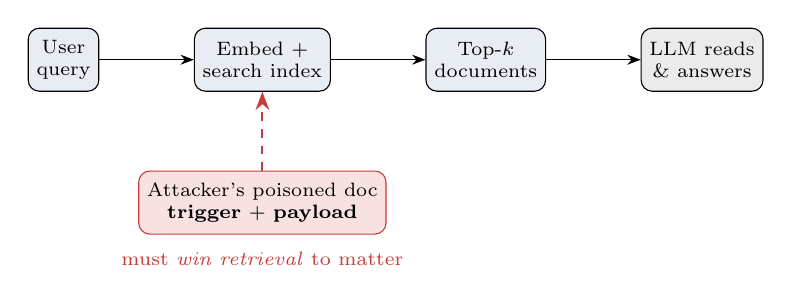
\begin{tikzpicture}[node distance=8mm and 12mm,
      box/.style={draw,rounded corners,align=center,font=\scriptsize,minimum height=8mm,inner sep=3pt},
      >={Stealth[]}]
    \node[box,fill=rbblue!10] (q) {User\\query};
    \node[box,fill=rbblue!10,right=of q] (emb) {Embed +\\search index};
    \node[box,fill=rbblue!10,right=of emb] (top) {Top-$k$\\documents};
    \node[box,fill=rbgray!12,right=of top] (llm) {LLM reads\\\& answers};
    \draw[->] (q)--(emb); \draw[->] (emb)--(top); \draw[->] (top)--(llm);
    \node[box,fill=rbaccent!15,draw=rbaccent,below=10mm of emb] (poison) {Attacker's poisoned doc\\ \textbf{trigger} $+$ \textbf{payload}};
    \draw[->,rbaccent,thick,dashed] (poison) to[out=90,in=-90] (emb);
    \node[font=\scriptsize,rbaccent,below=1mm of poison] {must \emph{win retrieval} to matter};
  \end{tikzpicture}
  \end{center}
  \begin{alertblock}{The Retrieval Barrier}
    A malicious document can hijack the assistant \emph{only if it is retrieved first}.
    \textbf{No retrieval $\Rightarrow$ no injection.} Retrieval is the security gate.
  \end{alertblock}
\end{frame}

\begin{frame}{Indirect Prompt Injection (IPI) and the two-part attack}
  \small
  \begin{columns}[T]
    \column{0.52\textwidth}
    \textbf{Indirect} prompt injection: the attacker never talks to the model. They plant instructions inside a document and wait for the AI to retrieve and read it.
    \vspace{0.6em}

    The poisoned document is split into two parts:
    \begin{itemize}
      \item \textbf{Trigger ($x$)} --- text tuned so the document \emph{gets retrieved} for natural queries.
      \item \textbf{Payload ($D_{adv}$)} --- the actual malicious instruction, executed once read.
    \end{itemize}
    \column{0.48\textwidth}
    \begin{block}{Threat model (this project)}
      \scriptsize
      \begin{itemize}
        \item \textbf{Black-box:} attacker only queries an embedding model from outside.
        \item No gradients, no model internals, no access to the full corpus.
        \item \textbf{Scope: retrieval-only} --- we measure whether the poison is \emph{retrieved}, the paper's security gate (no LLM/agent layer).
      \end{itemize}
    \end{block}
  \end{columns}
\end{frame}

% ===================================================================
\section{Motivation and Contribution}

\begin{frame}{Research gap: what is actually still open}
  \small
  We audited the source paper's claimed open problems against the literature.
  \begin{itemize}
    \item Several ``gaps'' are \textbf{already answered} or are restatements of the paper's own limitations.
    \item \good{Two gaps genuinely survive:}
      \begin{enumerate}
        \item \textbf{Provenance-aware retrieval} --- systems mostly ignore \emph{where} a document came from.
        \item \textbf{Query-distribution (T2) defenses} against an \emph{adaptive} attacker.
      \end{enumerate}
  \end{itemize}
  \begin{exampleblock}{Our contribution}
    A reproducible, CPU/GPU-portable testbed that (i) faithfully reproduces the black-box retrieval attack, (ii) extends it through a full hybrid + reranking pipeline, and (iii) introduces and evaluates a \textbf{provenance-weighted retrieval defense} --- the first of the two surviving gaps.
  \end{exampleblock}
\end{frame}

% ===================================================================
\section{The rbench Testbed}

\begin{frame}{System architecture: \texttt{rbench}}
  \small
  \begin{center}
  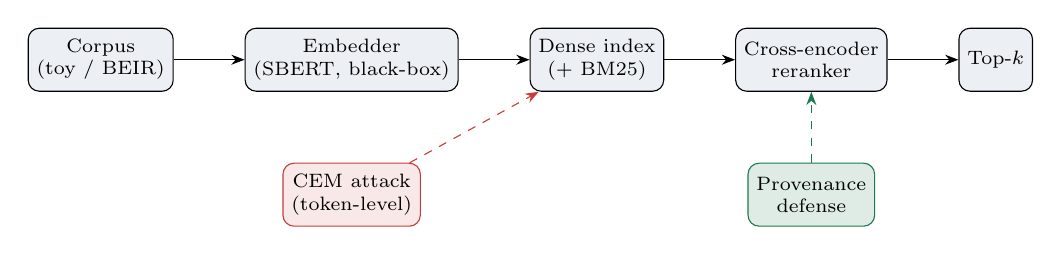
\begin{tikzpicture}[node distance=6mm and 9mm,
      b/.style={draw,rounded corners,align=center,font=\scriptsize,minimum height=8mm,inner sep=3pt,fill=rbblue!8},
      >={Stealth[]}]
    \node[b] (corp) {Corpus\\(toy / BEIR)};
    \node[b,right=of corp] (emb) {Embedder\\(SBERT, black-box)};
    \node[b,right=of emb] (idx) {Dense index\\(+ BM25)};
    \node[b,right=of idx] (rr) {Cross-encoder\\reranker};
    \node[b,right=of rr] (topk) {Top-$k$};
    \draw[->] (corp)--(emb); \draw[->](emb)--(idx); \draw[->](idx)--(rr); \draw[->](rr)--(topk);
    \node[b,fill=rbaccent!12,draw=rbaccent,below=9mm of emb] (atk) {CEM attack\\(token-level)};
    \node[b,fill=rbgreen!14,draw=rbgreen,below=9mm of rr] (def) {Provenance\\defense};
    \draw[->,rbaccent,dashed] (atk)--(idx);
    \draw[->,rbgreen,dashed] (def)--(rr);
  \end{tikzpicture}
  \end{center}
  \vspace{-0.3em}
  \begin{columns}[T]
    \column{0.5\textwidth}
    \textbf{Retrieval pipeline (switchable)}
    \begin{itemize}\scriptsize
      \item \emph{dense-only} --- the base paper's setting.
      \item \emph{hybrid} --- dense $+$ BM25 fused, then cross-encoder reranked.
    \end{itemize}
    \column{0.5\textwidth}
    \textbf{Engineering for scale}
    \begin{itemize}\scriptsize
      \item Honest corpus embedded \emph{once}; each poison trial re-embeds only the single poison doc.
      \item \texttt{--device auto} (CPU $\leftrightarrow$ GPU); reproducible on a Colab T4.
    \end{itemize}
  \end{columns}
\end{frame}

\begin{frame}{Evaluation setup}
  \small
  \begin{columns}[T]
    \column{0.5\textwidth}
    \textbf{Data}
    \begin{itemize}\scriptsize
      \item Real benchmark: \textbf{BEIR / SciFact} (5{,}000 scientific abstracts, 50 queries).
      \item Fetched directly from the official BEIR host; honest docs $=$ trusted KB.
    \end{itemize}
    \textbf{Models}
    \begin{itemize}\scriptsize
      \item Embedder: \texttt{all-MiniLM-L6-v2}; Reranker: \texttt{ms-marco-MiniLM}.
    \end{itemize}
    \column{0.5\textwidth}
    \textbf{Metrics}
    \begin{itemize}\scriptsize
      \item \textbf{RSR@$k$} (Retrieval Success Rate): fraction of target queries whose poison doc lands in the top-$k$ ($k{=}5$). \emph{Primary security metric.}
      \item \textbf{Honest recall@$k$:} corpus-health / utility check.
    \end{itemize}
    \textbf{Attack variants}
    \begin{itemize}\scriptsize
      \item \emph{none} (no trigger), \emph{naive} (echo the query), \emph{cem} (optimized).
    \end{itemize}
  \end{columns}
\end{frame}

% ===================================================================
\section{Phase 2: Reproducing the Attack}

\begin{frame}{The attack: black-box, token-level CEM}
  \small
  We optimize the trigger with the \textbf{Cross-Entropy Method} --- faithful to the authors' released method (independently implemented, no code reused).
  \begin{block}{CEM loop (per target query)}
    \scriptsize
    Maintain a per-position categorical distribution $P$ over the embedder's \textbf{token vocabulary}.
    \begin{enumerate}
      \item \textbf{Sample} a batch of candidate triggers (token sequences) from $P$.
      \item \textbf{Score} each by embedding similarity of (trigger $+$ payload) to the query.
      \item \textbf{Keep the elite} top fraction; \textbf{update} $P$ toward them (with smoothing).
      \item Repeat until convergence.
    \end{enumerate}
  \end{block}
  \vspace{-0.2em}
  \footnotesize Search space $=$ raw tokenizer tokens (the paper's actual method), not a curated word list --- triggers read as token fragments, not English.
\end{frame}

\begin{frame}{Phase 2 results --- SciFact (5{,}000 docs)}
  \small
  \begin{center}
  \begin{tabular}{lcc}
    \toprule
    \textbf{Poison variant} & \textbf{dense-only} & \textbf{hybrid $+$ rerank}\\
    \midrule
    none (no trigger)      & 0\%   & 0\% \\
    naive (echo the query) & 100\% & 100\% \\
    \textbf{cem (optimized)} & \bad{100\%} & \bad{72\%} \\
    \bottomrule
  \end{tabular}
  \end{center}
  \vspace{0.3em}
  Honest recall@5 $=$ \textbf{0.71} (a genuine, competitive retrieval setup).
  \begin{itemize}\small
    \item \good{Reproduced} the core result: no trigger $\to 0\%$; optimized trigger $\to 100\%$ on dense retrieval --- \textbf{the barrier is broken on purpose}.
    \item \textbf{Beyond the paper:} the same attack pushes through the full hybrid $+$ cross-encoder pipeline (\bad{72\%}); the reranker \emph{raises the attacker's budget, it is not a defense}.
  \end{itemize}
  \footnotesize\textcolor{rbgray}{Attacker is the black-box CEM optimizer; the trigger search now runs at the token level (the paper's exact method, independently implemented).}
\end{frame}

% ===================================================================
\section{Phase 3: Provenance-Weighted Defense}

\begin{frame}{A defense that ignores content and looks at \emph{origin}}
  \small
  Content-based ranking can always be gamed. Instead, weight documents by \textbf{provenance} (trust of their source):
  \[
    \text{score}'(d) \;=\; \text{score}(d) \;-\; \beta\,\bigl(1-\text{trust}(d)\bigr)\cdot(\text{score spread})
  \]
  \begin{columns}[T]
    \column{0.54\textwidth}
    \begin{itemize}\scriptsize
      \item trust: \texttt{internal} $=1$, \texttt{unknown} $=0.5$, \texttt{external} $=0$.
      \item $\beta$ tunes penalty strength; scaled to each pipeline's score range.
      \item Poison is \texttt{external} by construction.
    \end{itemize}
    \column{0.46\textwidth}
    \begin{alertblock}{Honesty guardrail}
      \scriptsize 30\% of the \emph{honest} corpus is legitimately \texttt{external}. The defense \textbf{cannot} just exclude all external docs --- it pays a real recall cost. This forces a genuine security/utility trade-off.
    \end{alertblock}
  \end{columns}
\end{frame}

\begin{frame}{Phase 3 results --- the security/utility trade-off}
  \small
  \begin{center}
  \begin{tabular}{ccccl}
    \toprule
    $\beta$ & \textbf{honest recall} & \textbf{RSR (naive)} & \textbf{RSR (cem)} & \\
    \midrule
    0.00 & 0.71 & 100\% & 100\% & \textcolor{rbgray}{no defense} \\
    0.25 & 0.52 & 94\%  & 86\%  & \\
    \rowcolor{rbgreen!12}
    0.50 & 0.50 & \good{8\%} & \good{6\%} & \textbf{sweet spot} \\
    0.75 & 0.50 & 0\%   & 0\%   & \\
    1.00 & 0.50 & 0\%   & 0\%   & \\
    \bottomrule
  \end{tabular}
  \end{center}
  \begin{itemize}\small
    \item At $\beta{=}0.5$: attack collapses \good{$100\%\!\to\!6\%$} for a bounded utility cost (recall $0.71\!\to\!0.50$).
    \item The recall floor $\approx 0.50$ is \emph{structural}: with 30\% of relevant docs external, you cannot both ingest untrusted content and be immune to it.
  \end{itemize}
\end{frame}

\begin{frame}{Key insight: source-based beats content-based}
  \begin{columns}[T]
    \column{0.5\textwidth}
    \begin{block}{Content-based (reranker)}
      \scriptsize
      Blunts the optimized \texttt{cem} attack ($100\%\!\to\!72\%$) but \textbf{not} the crude query-echo \texttt{naive} attack ($100\%$).\\[0.3em]
      $\Rightarrow$ \bad{attack-specific}: catches one trick, misses another.
    \end{block}
    \column{0.5\textwidth}
    \begin{exampleblock}{Source-based (provenance)}
      \scriptsize
      Collapses \texttt{naive} and \texttt{cem} \emph{together} ($\to 8\%/6\%$) --- it does not care \emph{how} the poison became relevant, only \emph{where it came from}.\\[0.3em]
      $\Rightarrow$ \good{attack-agnostic}.
    \end{exampleblock}
  \end{columns}
  \vspace{0.6em}
  \begin{center}
  \emph{The defense that ignores content is the one the attacker cannot out-optimize --- as long as trust labels hold.}
  \end{center}
\end{frame}

% ===================================================================
\section{Summary and Next Steps}

\begin{frame}{What we have done so far}
  \small
  \begin{itemize}
    \item \good{Phase 1 --- Testbed.} RAG retriever with switchable dense vs.\ hybrid $+$ reranker; incremental poison insertion for BEIR-scale corpora; reproducible on Colab GPU.
    \item \good{Phase 2 --- Attack.} Black-box, token-level CEM trigger optimizer (faithful to the USENIX'26 method). Reproduced $0\%\!\to\!100\%$ on dense; showed the reranker only reaches $72\%$ resistance.
    \item \good{Phase 3 --- Defense.} Provenance-weighted retrieval with an honest trade-off evaluation: $100\%\!\to\!6\%$ attack at a bounded recall cost; source-based defense generalizes across attacks where content-based defense does not.
    \item Full reproducibility: versioned repository, one-command Colab bootstrap.
  \end{itemize}
  \begin{block}{Relation to prior work}
    \scriptsize The authors released the \emph{attack} only (no defense). Our provenance defense and the planned adaptive attacker target the two \emph{surviving} gaps --- not covered by their artifact.
  \end{block}
\end{frame}

\begin{frame}{Next: Phase 4 --- the adaptive attacker}
  \small
  Our defense so far is tested against a \textbf{static} (defense-unaware) attacker. The real test:
  \begin{itemize}
    \item \textbf{Defense-aware, query-distribution (T2) attacker} --- optimize one trigger against the \emph{penalized} score over a distribution of queries; test on held-out queries.
    \item \textbf{Trust-inflation / spoofing} --- quantify how much attack success returns if the attacker can raise the poison's apparent trust (the real weak point of provenance).
    \item Report the three-column story: \emph{no defense} $\to$ \emph{defense (static)} $\to$ \emph{defense (adaptive)}.
  \end{itemize}
  \vspace{0.4em}
  Then: transferability across embedders, and a write-up positioning against Semantic Chameleon and CRCP.
\end{frame}

\begin{frame}[plain]
  \centering
  \vspace{1.5em}
  {\Large\color{rbblue}\textbf{Thank you}}\\[0.8em]
  \small Retrieval is the security frontier --- and a source-aware defense\\ is the piece the field is still missing.\\[1.2em]
  \footnotesize Sadman Bin Tareq (2105040) \quad$\cdot$\quad Rageeb Hasan Shafee (2105175)
\end{frame}

\end{document}
